\documentclass[11pt,twoside,a4paper]{article}
\usepackage{amsmath}
\usepackage{commath}
\usepackage{graphicx}

\begin{document}
\section{Uivariate Gaussian distribution}
  Let $\{x_i\}= \{x_1, x_2, \cdots,x_n\}$ denote $n$ random variates drawn from
  a univariate Normal distribution parametrised by the unknown variance $\omega$
  and known mean $\mu = 0$. Let us assume that the a Gaussian noise with known
  variannce $\zeta$ has been added to the variates yeilding new variates
  $\{y_i\}= \{y_1, y_2, \cdots,y_n\}$. Using statistical notations we can write
  \begin{align}
    \label{eqn_posteriors_signal_and_noise}
    \Pr \left(\{x_i\} | \omega \right) &= \prod_{i=1}^n
      \frac{1}{\sqrt{2 \pi \omega}} \exp \left(-\frac{x_i^2}{2 \omega} \right)\\
    \Pr \left(\{x_i\} | \{y_i\}, \zeta \right) &= \prod_{i=1}^n
      \frac{1}{\sqrt{2 \pi \zeta}} \exp
      \left(-\frac{\left(y_i - x_i \right)^2}{2 \zeta} \right)
  \end{align}
  Using Bayes theorem the inference about the variance $\omega$ can be written
  as
  \begin{align}
    \label{eqn_posterior_omega_given_noisy_random_variates}
    \Pr \left(\omega | \{y_i\} \right) \propto
      \Pr \left(\{y_i\} | \omega \right) \Pr(\omega).
  \end{align}
  Assuming a prior distribution $\Pr(\omega) = 1$, we can transfom the problem
  to the computation of the conditional distribution which is given by
  \begin{align}
    \Pr \left(\{y_i\} | \omega \right) &= \prod_{i=1}^n
      \frac{1}{\sqrt{2 \pi (\zeta + \omega)}} \exp
      \left(-\frac{y_i^2}{2(\zeta + \omega)} \right), \nonumber \\
    &= (2 \pi)^{-\frac{n}{2}} \left(\zeta + \omega \right)^{-\frac{n}{2}}
      \exp \left(-\frac{\sum_{i=1}^n y_i^2}{2 (\zeta + \omega)} \right) .
  \end{align}
  This equation represents an inverse-Gamma distribution:
  \begin{align}
    f(x | \alpha, \beta) = \frac{\beta^{\alpha}}{\Gamma(\alpha)} x^{\alpha - 1}
        \exp \left(-\frac{\beta}{x} \right).
  \end{align}
  The statistical properties of inverse-Gamma distribution is well known and
  are shown in the table below.
  \begin{table}
    \caption{Statistical properties of inverse-Gamma distribution}
    \label{tab_statistical_properties_of_inverse_gamma}
    \begin{center}
      \begin{tabular}{|c|c|c|}
        \hline
        mode & mean $(\alpha > 1)$ & variance $(\alpha > 2)$ \\
        \hline
        $\frac{\beta}{\alpha + 1}$ & $\frac{\beta}{\alpha - 1}$ &
          $\frac{\beta^2}{(\alpha - 1)^2 (\alpha - 2)}$ \\
        \hline
      \end{tabular}
    \end{center}
  \end{table}
  We can find the values of $n$ for which the variance of the distribution is
  defined as shown below:
  \begin{align}
    \alpha > 2 \\
    \frac{n}{2} + 1 > 2 \\
    \frac{n}{2} > 1 \\
    \boxed{n > 2}
  \end{align}
  This implies that we need at least 2 samples to determine the variance of the
  estimated and at least one sample to determine the mean.

  The logarithm of the posterior distribution can be written as
  \begin{align}
    \psi &= \log \left(\Pr \left(\{y_i\} | \omega \right) \right) \\
    &= -\frac{n}{2}\log(2 \pi) - \frac{n}{2}\log(\zeta + \omega)
      -\frac{1}{2} \frac{\sum_{i=1}^n y_i^2}{(\zeta + \omega)}.
  \end{align}
  The gradient of the log-posterior with respect to $\omega$ is given by
  \begin{align}
    \frac{\partial \psi}{\partial \omega} = -\frac{n}{2 (\zeta + \omega)}
      - \frac{\sum_{i=1}^n y_i^2}{2 (\zeta + \omega)^2}.
  \end{align}
  The mode of the distribution can be found by setting gradients equal to zero
  and solving the resulting equation:
  \begin{align}
    \frac{n}{2 (\zeta + \omega)}
      + \frac{\sum_{i=1}^n y_i^2}{2 (\zeta + \omega)^2} = 0, \\
    \frac{n}{2} + \frac{\sum_{i=1}^n y_i^2}{2 (\zeta + \omega)} = 0 \\
    n + \frac{\sum_{i=1}^n y_i^2}{(\zeta + \omega)} = 0 \\
    n (\zeta + \omega) + \sum_{i=1}^n y_i^2 = 0
    %\zeta + \omega + \frac{\sum_{i=1}^n y_i^2}{n} = 0 \\
    %\omega = \frac{\sum_{i=1}^n y_i^2}{n} - \zeta \\
    %\omega = \bar{y} - \zeta
  \end{align}
  Thus mode of the distribution is given by
  \begin{align}
    \boxed{\bar{\omega} = \bar{y} - \zeta.}
  \end{align}
  As we can see, the mode may have chance of being negative or zero which
  corresponds to non-physical variance. Hence we cannot treat this as point
  estimate of the distribution. The question then is what suffices as a
  ``good'' point estimate?

  From a Bayesian prespective, we haven't really assed the situaton carefully.
  By choosing uniform prior for $\omega$ we have allowed non-positive values
  for the variance. However, a sensible prior for the variance should disregard
  any values less than or equal to zero. According to Jeffery's a reasonable
  prior distribution for a variable taking only positive values should be
  a uniform prior on the logarithm of the variable. Let $\eta = \log(\omega)$
  and hence we can write,
  \begin{align}
    \Pr(\eta) = 1.
  \end{align}
  The rule of chang of variables says that
  \begin{align}
    \Pr(\omega) \dif \omega = \Pr(\eta) \dif \eta.
  \end{align}
  Therefore the Jeffreys prior on $\omega$ can be derived as
  \begin{align}
    \Pr(\omega) &= \Pr(\eta) \frac {\dif \eta}{\dif \omega}, \\
    &= \frac{1}{\omega}.
  \end{align}

  Applying the Jeffreys prior, the logarithm of the posterior distribution
  becomes
  \begin{align}
    \psi  = - \frac{n}{2} \log (2 \pi) - \frac{n}{2} \log (\zeta + \omega)
      - \frac{1}{2} \frac{\sum_{i=1}^n y_i^2}{(\zeta + \omega)} - \log(\omega).
  \end{align}
  We compare the two posterior distributions in
  Figure~\ref{fig_log_post_uniform_jeffreys}
  \begin{figure}
    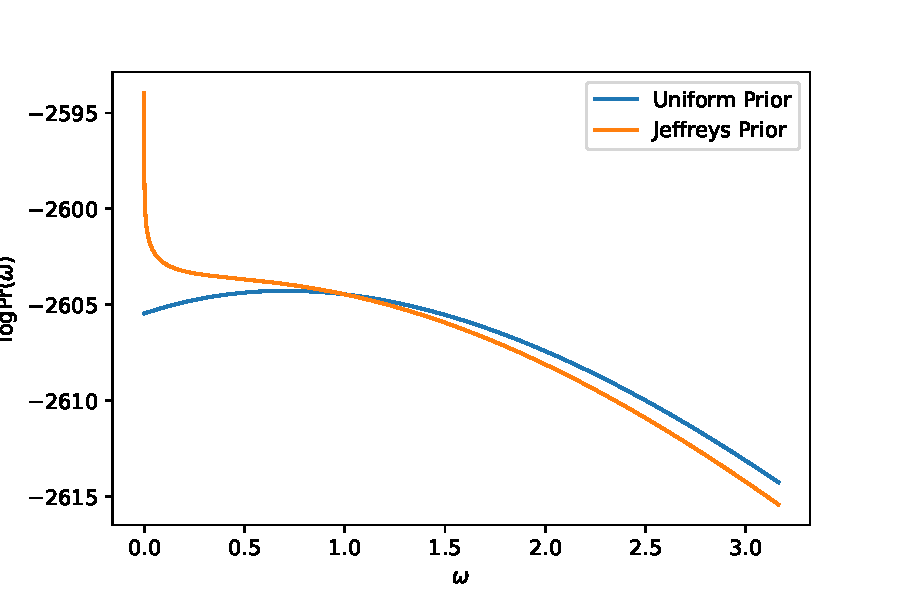
\includegraphics[scale=0.8]{images/log_post_uniform_jeffreys.pdf}
    \caption{Comparing the log-posterior distributions of $\omega$ with uniform and Jeffreys prior.}
    \label{fig_log_post_uniform_jeffreys}
  \end{figure}

\end{document}
